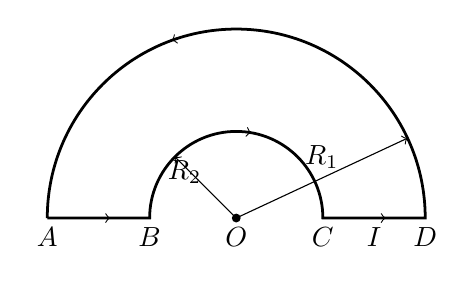
\begin{tikzpicture}
\def\a{2.4}\def\b{1.1}
\draw[line width=1pt] (-\a,0) -- (-\b,0) arc[start angle=180,end angle=0,radius=\b] -- (\a,0) arc[start angle=0,end angle=180,radius=\a];
\draw[->] (-1.9,0) -- (-1.6,0); \draw[->] (1.6,0) -- (1.9,0); \draw[->] (100:\a) arc[start angle=100,end angle=110,radius=\a]; \draw[->] (100:\b) arc[start angle=100,end angle=80,radius=\b];
\fill (0,0) circle (1.6pt) node[below]{$O$}; \draw[->] (0,0) -- node[above left=-2pt]{$R_2$} (135:\b); \draw[->] (0,0) -- node[above]{$R_1$} (25:\a);
\foreach \x/\l in {-2.4/A,-1.1/B,1.1/C,2.4/D} \node[below] at (\x,0) {$\l$}; \node[below] at (1.75,0) {$I$};
\end{tikzpicture}
